\documentclass[a4paper,12pt]{article}
\usepackage[polish]{babel}
\usepackage[utf8]{inputenc}
\usepackage[T1]{fontenc}
\usepackage{indentfirst}
\usepackage[top=2.5cm, bottom=2.5cm, left=2.5cm, right=2.5cm]{geometry}
\usepackage{amsmath}
\usepackage{hyperref}
\usepackage{enumerate}
\usepackage{graphicx}

\title{Symulacja rozprzestrzeniania dymu}
\author{Autorzy: Michał Kowalczyk, Kacper Kontny, Denis Lyakhov}
\date{\today}
\begin{document}
	\maketitle
	
	\section{Cele}
	\begin{enumerate}[i.]
	    \item Głównym zadaniem w tym projekcie jest stworzenie trójwymiarowego modelu rozprzestrzeniania się dymu w pomieszczeniu.
        \item Model powinien uwzględniać takie czynniki jak temperaturę czy kierunek ruchu powietrza.
        \item W ramach projektu należy opracować model i przygotować symulację 3D.
	\end{enumerate}

	
	\section{Wprowadzenie}
	
	
	Większość nowoczesncyh metod symulacji nie tylko dymu, ale też gazów i
	płynów są oparte na tzw. równaniu Naviera-Stokes'a. Za ich pomocą można symulować rozprzestrzenianie się cieczy i gazów w 2D i 3D.
	
	\vspace{5mm}
	
	Równanie Navier-Stokes'a - w mechanice płynów - równanie różniczkowe
	cząstkowe, opisujące fizykę cieczy. Mówiąc dokładniej, opisuje
	zmianę prędkości przepływu w czasie. Mając aktualny stan prędkości i zbiór sił, rownania te mogą nam powiedzieć dokładnie, jak zmienia się prędkość w każdym nieskończenie małym przedziale czasu.
	
	Równania Navier-Stokes'a wyglądają następująco:
	
	\begin{equation}
	    \frac{\partial u}{\partial t} = -(u \cdot \nabla)u+\nu\nabla^{2}u+f
	\end{equation}
	
	\begin{equation}
	    \frac{\partial \rho}{\partial t}=-(u\cdot\nabla)\rho+\kappa\nabla^{2}\rho + S
	\end{equation}
	
	\vspace{5mm}

	Pierwsze równanie opisuje zmianę prędkości, a drugie - gęstości.
	
	\vspace{5mm}
	
	Aby mieć możliwość rozwiązywania takich równań w czasie rzeczywistym,
	posługujemy algorytmami numerycznymi.
	
	\vspace{5mm}
	
	Ale mamy problem. Chociaż możemy przewidzieć zachowanie się prędkości
	przepływu cieczy w nieskońcenie małych przedziałach czasu, w praktyce we
	współczesnym świecie nie dysponujemy (i raczej nigdy nie będziemy)
	komputerami, posiadającymi moc obliczeniową wystarczającą do obliczenia
	zachowania się każdej małej cząstecki płynu albo gazu na poziome
	molekularnym. W związku z tym, aby rozwiązać ten problem musimy
	zoptymalizować naszą symulację.
	
	\vspace{5mm}
	
	Zamiast milionów cząsteczek dymu, nasza
	symulacja komputerowa będzie posiadać siatkę ze skończoną liczbą komórek.
	Gęstość i prędkość każdej "części" naszego dymu zostaną zapisane w środku
	każdej z naszych komórek (rys. 1).
	
    \vspace{5mm}
    
    W taki sposób znacznie zmniejszymy obciążenia obliczeniowe,
    co pozwoli nam na urochomienie symulacji w czasie rzeczywistym.
    
    \begin{figure}
    \centerline{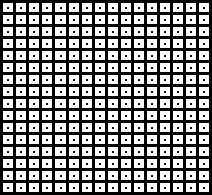
\includegraphics[scale=2]{grid2.png}}
    \caption{Siatka 2D N*N}
    \label{fig:siatka2d}
    \end{figure}
	
	
	\section{Tytuł}
	Tekst tytułu
	
	
	\pagebreak
	\begin{thebibliography}{15}
	
	    \bibitem{id}
		Eren Algan, \textit{REAL-TIME SMOKE SIMULATION},
		\texttt{\href{http://repository.bilkent.edu.tr/bitstream/handle/11693/15609/0006332.pdf?sequence=1&isAllowed=y}{link}}.
		
		\bibitem{id}
		Jos Stam, \textit{Real-Time Fluid Dynamics for Games}.
		
		\bibitem{id}
		Marinus Rorbech, \textit{REAL-TIME SIMULATION OF SMOKE USING GRAPHICS HARDWARE},
		\texttt{\href{http://image.diku.dk/projects/media/roerbech.04.pdf}{link}}.
		
		\bibitem{id}
		Ronald Fedkiw, Jos Stam, Henrik Wann Jensen, \textit{Visual Simulation of Smoke},
		\texttt{\href{http://graphics.ucsd.edu/~henrik/papers/smoke/smoke.pdf}{link}}.
		
		\bibitem{id}
		Michael Ash, \textit{Simulation and Visualization of a 3D Fluid},
		\texttt{\href{https://www.mikeash.com/thesis/thesis-en.pdf}{link}}.
		
	\end{thebibliography}
	
\end{document}
